\documentclass[journal]{IEEEtran}

% *** CITATION PACKAGES ***
\usepackage{cite}

% *** GRAPHICS RELATED PACKAGES ***
\usepackage{graphicx}
\graphicspath{{figures/}{./figures/}{../figures/}}
\DeclareGraphicsExtensions{.pdf,.jpeg,.png,.eps}

% *** MATH PACKAGES ***
\usepackage{amsmath,amssymb,amsfonts}

% *** TABLE PACKAGES ***
\usepackage{booktabs}
\usepackage{multirow}
\usepackage{array}

% *** URL AND HYPERLINK PACKAGES ***
\usepackage{url}
\providecommand{\doi}[1]{\url{https://doi.org/#1}}

% *** TYPOGRAPHY ***
\usepackage[T1]{fontenc}
\usepackage{microtype}

\begin{document}

\title{Efficient Brain MRI Classification with Sub-1M Parameter Models and Multi-Scale Consistency-Guided Inference}

\author{Anonymous~Authors%
\thanks{Manuscript draft submitted for peer review. Code, configs, and pre-trained weights will be made publicly available upon publication.}}

\markboth{IEEE Transactions on Medical Imaging,~Draft~Manuscript,~October~2026}%
{Anonymous Authors: Efficient Brain MRI Classification with Sub-1M Parameter Models}

\maketitle
\begin{abstract}
Deep learning has transformed medical image analysis, becoming central to many clinical applications. However, real-world deployment remains challenging due to computational demands, latency constraints, and privacy concerns associated with cloud-based processing. Despite these limitations, state-of-the-art models increasingly favor larger architectures and datasets, reinforcing a scale-driven paradigm that is often impractical for resource-constrained systems.

This study systematically evaluates deep learning models with fewer than one million parameters on small-to-medium-sized datasets for image classification and detection, focusing on efficiency and cross-dataset generalization. Results show that on saturated classification benchmarks, compact models can achieve performance statistically comparable to models an order of magnitude larger. The best model attains 98.3\% accuracy at 0.36 GFLOPs, running six times faster with less than a one-percentage-point accuracy difference. However, a performance gap remains on more challenging cross-dataset tasks, with errors concentrated in low-confidence predictions sensitive to input perturbations. The most efficient architecture, which uses parallel atrous convolution branches to capture multi-scale features, is particularly vulnerable to scale-sensitive inputs.

To address this limitation, we propose \textbf{MCG-TTA}, an architecture-informed inference strategy designed to improve robustness while limiting computational overhead. MCG-TTA improves slice-level F1 by up to 1.8 percentage points at approximately 1.9$\times$ the baseline latency, while retaining a model size of 0.91 million parameters. These findings suggest that, for resource-constrained clinical applications, uncertainty-aware inference can recover residual accuracy more efficiently than increasing model complexity.
\end{abstract}

\begin{IEEEkeywords}
Brain MRI, convolutional neural networks, compact neural networks, test-time augmentation, glioma grading, edge inference.
\end{IEEEkeywords}

\IEEEpeerreviewmaketitle

\section{Introduction}
\IEEEPARstart{D}{eep} Neural Networks (DNNs) have established foundational breakthroughs across core computer vision tasks, ranging from large-scale visual recognition \cite{8, 19} to dense spatial reasoning and object detection \cite{10, 37}. This technological trajectory was initially catalyzed by Convolutional Neural Networks (CNNs) \cite{15, 18}, which embedded translation equivariance and localized hierarchies into learnable architectures. To overcome gradient degradation in deeper layers, residual connections \cite{10} and compound scaling principles \cite{30} subsequently enabled networks to scale in depth and width. In recent years, the visual landscape has experienced an additional paradigm shift toward Vision Transformers (ViTs) \cite{6, 33}, masked image modeling \cite{34}, and self-supervised foundation backbones \cite{1}. While relaxing convolutional inductive biases enables dynamic global contextual reasoning, modern progress has predominantly reinforced an unsustainable ``scale-driven'' paradigm \cite{32}: marginal benchmark gains are increasingly acquired by expanding architectures to tens or hundreds of millions---and increasingly billions---of parameters over colossal compute clusters and proprietary web-scale datasets \cite{8, 32} (as analyzed across dominant paradigms in Section~\ref{sec:related_work}).

In parallel with these computational trends, deep learning has profoundly influenced clinical radiology, demonstrating diagnostic efficacy competitive with subspecialized clinicians across diverse imaging modalities \cite{7, 28}. Within neuro-oncology, non-invasive Magnetic Resonance Imaging (MRI) serves as the definitive clinical modality for the screening, differential diagnosis, and histologic grading of intracranial neoplasms \cite{2, 26, 38}. Clinical decision-making requires precise differentiation among distinct pathological entities---primarily diffuse infiltrative gliomas, extra-axial dural meningiomas, and sellar pituitary adenomas---as each exhibits vastly disparate treatment pathways ranging from urgent surgical resection and chemoradiotherapy to conservative observation \cite{26, 40}. Radiologically, this differential triage demands meticulous evaluation of subtle cytoarchitectural hallmarks: discerning irregular invasive margins from well-circumscribed borders, characterizing microvascular permeability and blood-brain barrier disruption, and distinguishing non-enhancing infiltrative edema from central necrotic cores across multi-parametric acquisitions (including T1-weighted, contrast-enhanced T1ce, T2-weighted, and FLAIR sequences) \cite{2, 28, 38}. However, manual multi-planar slice inspection across axial, coronal, and sagittal volumes imposes immense cognitive burdens on neuroradiologists, creating clinical vulnerability to intra- and inter-observer diagnostic variability and triage delays \cite{7, 40}. To automate the detection of these complex radiological phenotypes, prevailing medical imaging pipelines have routinely transposed off-the-shelf, overparameterized computer vision backbones into clinical workflows \cite{7, 39, 40}, inadvertently importing their extreme memory and computational footprints into hospital environments.

Despite these empirical successes, a critical translational divide persists between benchtop benchmark accuracy and clinical, point-of-care utility \cite{21, 25}. In healthcare environments, real-world deployment rarely occurs in centralized, high-throughput cloud data centers. Routine transmission of high-resolution volumetric neuroimaging to external cloud infrastructures encounters severe regulatory barriers, notably patient confidentiality mandates and data protection governance such as HIPAA in the United States and GDPR in the European Union \cite{21}. Furthermore, cloud dependency introduces vulnerability to variable network bandwidth, transmission latency, and service outages---risks that are unacceptable during acute clinical scenarios, emergency neuro-triage, or intra-operative surgical navigation \cite{21, 25}. Consequently, bringing intelligence directly to the clinical edge---operating locally on hospital workstations, embedded scanner consoles, and mobile intra-operative carts---has emerged as an urgent imperative \cite{9, 20, 21}.

However, edge deployment imposes uncompromising physical constraints: strict inference latency windows, severely constrained Random Access Memory (RAM), low thermal design power (TDP), and limited on-chip arithmetic hardware \cite{9, 25}. To accommodate mobile and decentralized environments, the vision community introduced lightweight architectural designs \cite{22} (detailed in Section~\ref{sec:related_work}), including depthwise separable convolutions \cite{11, 27}. Yet, the overwhelming majority of these ``efficient'' models predominantly inhabit a mobile-scale budget of 2 to 20 million parameters. In contrast, the sub-1M parameter regime ($<1,000,000$ parameters) remains fundamentally underexplored in medical imaging, particularly under the practical constraints of small-to-medium institutional datasets \cite{3, 16}. Crucially, as observed in recent foundational studies on compact architectures \cite{16}, naively downscaling standard architectures via uniform width or depth multipliers leads to erratic representational capacity, gradient instability, and disproportionate performance collapse \cite{16, 19}.

This investigation is motivated by the absence of systematic benchmarks, architectural insights, and deployment guidelines for deep learning models operating under a strict sub-1M parameter ceiling in neuro-oncological imaging. We posit that as the parameter budget is aggressively constrained, architectural topology---specifically how parameters are structurally allocated to capture multi-scale context without parameter redundancy---matters far more than sheer parameter volume \cite{16}. While multi-path atrous (dilated) depthwise convolutions have emerged as a premier mechanism for expanding effective receptive fields without parameter inflation \cite{5, 16}, their behavior, domain robustness, and failure mechanics under clinical distribution shifts have never been systematically characterized.

To address these foundational questions, this work presents a systematic empirical evaluation of deep learning models operating under a strict sub-1M parameter budget across representative neuro-oncological imaging tasks. Our empirical findings uncover two fundamental phenomena:
\begin{enumerate}
\item \textbf{In-Domain Saturation}: On canonical diagnostic benchmarks, architecturally optimized compact models match the diagnostic capability of overparameterized backbones an order of magnitude larger, while offering substantially faster inference speeds on unaccelerated edge processors. This demonstrates that for constrained clinical cohorts, high parameter capacity often yields diminishing returns.
\item \textbf{Cross-Dataset Multi-Scale Vulnerability}: When evaluated under out-of-domain clinical shifts, this saturation breaks. We find that compact models relying on parallel atrous convolutions become brittle under input scale perturbations, with predictive uncertainty concentrating along ambiguous lesion boundaries.
\end{enumerate}

In resource-constrained healthcare environments, resorting to larger models or heavy ensemble backbones to mitigate domain fragility is practically impermissible due to strict latency and memory limits \cite{9, 16}. Instead, we show that this residual accuracy gap can be recovered far more efficiently at inference time by leveraging the model's own architectural inductive biases. To this end, we introduce \textbf{Multi-Scale Consistency Gated Test-Time Augmentation (MCG-TTA)}. Rather than performing costly, unconditional multi-view inference across every image \cite{4, 35}, MCG-TTA monitors prediction uncertainty and selectively triggers targeted scale augmentations that align with the network's internal receptive field structure only when scale disagreement is detected, requiring zero additional learned parameters.

Extensive evaluations confirm that uncertainty-aware test-time calibration stabilizes compact representations under distribution shifts while preserving patient-level diagnostic reliability. These results demonstrate that architecture-informed inference calibration offers a practical, hardware-friendly alternative to model scaling for clinical edge artificial intelligence.

In summary, the principal contributions of this work are:
\begin{itemize}
\item \textbf{Systematic Sub-1M Benchmark and Edge Profiling}: We provide a comprehensive evaluation of sub-1M parameter vision architectures on neuro-oncological imaging, analyzing trade-offs across model capacity, real-device edge CPU latency, throughput, and cross-cohort generalization against mobile and overparameterized baselines, complemented by patient-level clinical sensitivity analysis.
\item \textbf{Characterization of Saturation and Domain Vulnerabilities}: We identify the saturation behavior of compact networks on in-domain medical diagnosis, and formally uncover the scale-sensitivity mechanics of compact atrous convolutions under clinical distribution shifts.
\item \textbf{Architecture-Informed Test-Time Inference}: We introduce MCG-TTA, a parameter-free, uncertainty-gated inference framework that dynamically stabilizes scale-sensitive compact representations at test time with minimal latency overhead.
\end{itemize}


\section{Related Work}
\label{sec:related_work}

Deep neural networks have catalyzed significant progress in medical computer vision, yet their deployment in real-time neuro-oncology remains severely hindered by the compute, memory, and latency bottlenecks of prevailing architectures. In this section, we review relevant literature across dominant architectural paradigms, examining their mathematical foundations, adoption in brain MRI diagnosis, and intrinsic operational limitations on resource-constrained clinical hardware.

\subsection{Residual Networks and the Computational Cost of Scale}
As convolutional neural networks grew deeper, optimization became increasingly hindered by vanishing and exploding gradients, as well as degradation where accuracy saturates and abruptly drops. He \emph{et~al.} \cite{10} resolved this degradation phenomenon with the Residual Network (ResNet), introducing identity shortcut connections that allow forward activations and backward error signals to bypass parameterized convolutional layers without attenuation. In clinical neuro-oncology, deep residual architectures---predominantly ResNet-18, ResNet-50, and ResNet-101---have established themselves as the standard backbone across tumor detection, multi-class classification, and histologic glioma grading \cite{7, 28, 38, 39}. Extensive surveys by Litjens \emph{et~al.} \cite{7} and Lundervold and Lundervold \cite{38}, together with benchmark studies such as Nayak \emph{et~al.} \cite{39}, demonstrate that deep CNNs---via ImageNet transfer learning or custom architectures---achieve near-saturated diagnostic accuracies (97.5--100\%) on multi-class brain MRI benchmarks \cite{39}, a saturation regime also consistently reproduced on public cohorts such as the Nickparvar dataset \cite{26}.

Despite their high benchmark accuracy, deep residual networks introduce acute operational liabilities in clinical practice. In original architectural specifications and comprehensive benchmarks by He \emph{et~al.} \cite{10} and Bianco \emph{et~al.} \cite{43}, standard ResNet-50 contains approximately 25.56 million parameters, requiring roughly 98 to 102 megabytes of storage for uncompressed single-precision weights alone, while VGG-16 \cite{29} comprises upwards of 138 million parameters (and over 27 million even when dense classification heads are trimmed). In terms of arithmetic complexity, a standard single-image forward pass through ResNet-50 requires 3.8 to 4.1 GFLOPs (roughly 3.86 to 4.09 GMACs) \cite{10, 43}, whereas VGG-16 demands over 15.3 GMACs (exceeding 30 GFLOPs) \cite{29, 43}. As documented in a comprehensive survey of deep learning on CPUs by Mittal \emph{et~al.} \cite{25}---with deployment constraints similarly noted in neuro-oncology imaging surveys \cite{40}---hospital workstations and portable intra-operative scanners rely primarily on general-purpose central processing units (CPUs) or low-power embedded processors lacking high-end enterprise GPU acceleration. On such resource-constrained hardware, deep residual backbones encounter severe latency bottlenecks: empirical benchmarking across embedded and edge platforms by Bianco \emph{et~al.} \cite{43} reveals that ResNet-50 is throttled to under 19 frames per second, with single-image inference latency frequently exceeding 50 to 80 milliseconds on unaccelerated consumer CPUs \cite{25, 44}. For clinical 3D MRI examinations containing hundreds of volumetric slices across multiple modalities (T1, T1Gd, T2, FLAIR) \cite{2, 23, 45}, this computational overhead translates into cumulative multi-second delays per patient, impeding emergency neuro-triage and interactive intra-operative navigation. Furthermore, empirical profiling demonstrates that the multi-branch bottleneck topology of ResNets incurs substantial Memory Access Cost (MAC) and off-chip DRAM memory traffic, generating severe cache thrashing that causes real-world hardware execution time to deviate unfavorably from theoretical FLOP estimates \cite{25}.

\subsection{Factorized Convolutions: Inverted Residuals and Linear Bottlenecks}
To provide computationally lightweight models capable of real-time execution on constrained hardware, depthwise separable convolutions were popularized by Chollet \cite{13} in Xception and generalized by Howard \emph{et~al.} \cite{11} in MobileNet. This decomposition decouples spatial filtering from channel mixing: a depthwise convolution applies a single spatial kernel per input channel, followed by a $1\times1$ pointwise convolution that linearly combines features across channels. For $3\times3$ kernels, this factorization achieves an 8- to 9-fold reduction in arithmetic operations with minimal loss of representational capacity. Sandler \emph{et~al.} \cite{27} introduced MobileNetV2, pioneering the inverted residual block with a linear bottleneck. Unlike conventional residual blocks that compress feature dimensions before spatial convolution, MobileNetV2 expands low-dimensional input features to a higher-dimensional intermediate space using pointwise convolutions, performs spatial depthwise filtering, and subsequently projects features back to a lower-dimensional manifold via a linear bottleneck to prevent non-linear activation collapse. MobileNetV3 \cite{14} enhanced this framework by pairing neural architecture search (NAS) \cite{36} with hardware-aware optimization, integrating hard-swish non-linearities and selective Squeeze-and-Excitation (SE) channel recalibration blocks \cite{12} to dynamically reweight feature maps according to global context.

\subsection{Principles of Compound Network Scaling}
The EfficientNet family \cite{30} was formulated to systematically balance accuracy and computational demand by rethinking network scaling. Prior works typically scaled a single dimension---either network depth, channel width, or input image resolution---in isolation. Tan and Le demonstrated that these three dimensions are fundamentally interdependent and introduced a principled compound scaling method that uniformly scales depth, width, and resolution using a fixed compound coefficient, effectively constraining target multiply-accumulate operations (MACs). EfficientNet-B0 serves as the baseline, operating at 5.3 million parameters and 0.39 GMACs \cite{30}. To resolve training latency bottlenecks and reduce memory overhead, EfficientNetV2 \cite{31} incorporated Fused-MBConv blocks, replacing early depthwise separable blocks with standard $3\times3$ convolutions to better exploit hardware acceleration and memory locality on modern CPUs and GPUs, while employing progressive learning strategies.

\subsection{Vision Transformers and Modernized Convolutional Networks}
Moving beyond pure convolutional inductive biases, the Vision Transformer (ViT) \cite{6} tokenizes images into discrete coordinate patches and applies global self-attention mechanisms \cite{33}. While ViTs exhibit exceptional representational capacity when pre-trained on web-scale datasets, their lack of translational equivariance and local inductive priors makes them notoriously prone to severe overfitting when trained from scratch on small-to-medium-scale medical cohorts \cite{19}. Furthermore, the quadratic computational complexity of pairwise global self-attention with respect to token length imposes prohibitive latency and memory footprints during high-resolution volumetric MRI processing \cite{6, 46}. Motivated by transformer advancements, Liu \emph{et~al.} \cite{24} introduced ConvNeXt, modernizing classic ResNets by incorporating large $7\times7$ kernels, inverted bottleneck designs, depthwise convolutions, and LayerNorm to achieve transformer-competitive performance while retaining the hardware efficiency and simplicity of ConvNets. ConvNeXt V2 \cite{34} combined this architecture with masked autoencoders and global response normalization to stabilize feature representation learning.

\subsection{Multi-Scale Feature Representation and Dilated Convolutions}
Discriminating diffuse intracranial tumor boundaries, perifocal vasogenic edema, and necrotic cores requires capturing spatial context across heterogeneous scales \cite{2, 23, 39}. Standard CNNs capture multi-scale context by progressively downsampling feature maps, sacrificing spatial boundary precision. In contrast, atrous (dilated) convolutions \cite{5} expand the effective receptive field without spatial resolution reduction or parameter inflation by introducing an integer dilation rate that spaces out kernel filter weights. Chen \emph{et~al.} \cite{5} popularized this concept through Atrous Spatial Pyramid Pooling (ASPP) in DeepLab, deploying parallel atrous convolutional branches with distinct dilation rates to capture multi-scale representations simultaneously. Kyrkou and Theocharides \cite{17} utilized multi-scale atrous fusion in EmergencyNet to achieve real-time aerial classification. Building upon these principles, Kyrkou \cite{16} introduced LiteSpeed-Net (LS-Net), demonstrating that multi-path atrous convolutions provide a potent inductive bias for compact vision models operating under a sub-1M parameter budget: by splitting channels across parallel depthwise branches with dilation rates of 1, 2, and 3, LS-Net achieves broad multi-scale receptive field coverage while maintaining high inference speed. However, multi-path atrous convolutions suffer from an unaddressed vulnerability in clinical neuro-imaging: because dilated kernels sample the spatial grid at rigid, discrete intervals without spatial interpolation \cite{5, 16}, their predictions become disproportionately fragile under input scale variations and cross-institution acquisition shifts, such as varying slice thickness and lesion zoom levels.

\subsection{Test-Time Augmentation and Aleatoric Uncertainty Estimation}
In safety-critical clinical applications, deep models must communicate predictive uncertainty alongside raw class scores \cite{7, 41}. In neuro-oncology MRI, diagnostic ambiguity arises from anatomical heterogeneity, scanner noise, and indistinct lesion margins---collectively defined as data-dependent aleatoric uncertainty \cite{4, 35}. Seminal works by Ayhan and Berens \cite{4} and Wang \emph{et~al.} \cite{35} demonstrated that Test-Time Augmentation (TTA) provides an effective Monte Carlo sampling framework to estimate aleatoric uncertainty without requiring Bayesian retraining. By applying a distribution of stochastic geometric and photometric transformations to a query slice at test time and averaging the resulting predictions, TTA smooths the decision boundary and yields calibrated uncertainty estimates \cite{4, 35, 42}. Nevertheless, conventional TTA introduces a severe computational bottleneck for edge deployment: running an unselective multi-view ensemble (e.g., 6 to 8 forward passes per image) multiplies inference latency by an equivalent linear factor \cite{42}. In clinical edge workflows, executing an unconditional multi-view TTA scales latency linearly with the number of augmentation passes, completely negating the execution speedups attained through compact architecture design \cite{35, 42}. Furthermore, as shown by Shanmugam \emph{et~al.} \cite{42}, unconditionally augmenting unambiguous high-confidence samples can distort canonical anatomical orientations, inadvertently corrupting diagnostic accuracy.

\subsection{Critical Gaps in Edge Neuro-Oncological Vision}
A critical synthesis of existing literature exposes three fundamental voids that motivate this investigation. First, prior medical imaging studies focus almost exclusively either on overparameterized backbones exceeding 20 million parameters (ResNet-50, VGG-16) or mobile-scale models (2M to 20M parameters). The strict sub-1M parameter regime ($<1,000,000$ parameters)---which represents the critical threshold for low-power microcontroller deployment, zero-latency caching, and localized hospital workstation integration---remains unbenchmarked across in-domain classification and out-of-domain clinical grading. Second, while parallel atrous convolutions achieve high efficiency on saturated in-domain benchmarks, their discrete sampling mechanics induce acute vulnerability to cross-dataset scale shifts, where diagnostic errors concentrate in low-confidence predictions near lesion boundaries. Third, existing test-time augmentation pipelines operate as unselective, brute-force ensembles that impose prohibitive latency penalties. No prior methodology leverages predictive uncertainty to selectively trigger TTA while matching the test-time transformations to the internal multi-scale receptive fields of compact atrous architectures.

To resolve these limitations, this paper establishes a systematic sub-1M benchmark on brain MRI diagnosis and introduces Multi-Scale Consistency Gated Test-Time Augmentation (MCG-TTA), recovering out-of-domain clinical accuracy with zero additional learned parameters while preserving edge-level inference speed.


\section{Methodology: Uncertainty-Gated Multi-Scale Inference (MCG-TTA)}

Motivated by the computational and latency constraints of clinical edge devices \cite{9, 20, 21}, and the observation that compact convolutional architectures relying on parallel dilated convolutions can exhibit sensitivity to input scale variations \cite{5, 16}, this work introduces \textbf{Multi-Scale Consistency Gated Test-Time Augmentation (MCG-TTA)}. The underlying hypothesis is that scale-induced ambiguity in compact multi-dilation models concentrates in low-confidence predictions, and that these predictions can be dynamically stabilized at inference time by probing the model with multi-scale views aligned with its internal dilation structure---requiring zero additional learned parameters.

In this section, we formulate the general image classification problem and base model representation, analyze the theoretical scale sensitivity of compact atrous convolutions, present the formal algorithmic pipeline of MCG-TTA across its three decision stages, derive an analytical edge latency model, and define the volumetric patient-level diagnostic aggregation.

\subsection{Problem Formulation and Base Network Representation}

Let $\mathbf{I} \in \mathbb{R}^{H \times W \times C}$ denote a 2D brain MRI slice, where $H, W$ represent spatial dimensions and $C$ denotes channel dimensionality. A deep neural network $f_\theta$ parameterized by learned weights $\theta$ maps the input slice to a vector of logits $\mathbf{z} = f_\theta(\mathbf{I}) \in \mathbb{R}^K$ over $K$ mutually exclusive diagnostic categories. 

The predicted class posterior probabilities are computed via the softmax operator:
\begin{equation}
\mathbf{p} = \sigma\left(f_\theta(\mathbf{I})\right) \in \Delta^{K-1}, \quad \text{where } p_c = \frac{\exp(z_c)}{\sum_{j=1}^K \exp(z_j)}
\label{eq:softmax}
\end{equation}
The model's predictive confidence is quantified by the maximum posterior probability:
\begin{equation}
p_{\max} = \max_{c \in \{1, \dots, K\}} p_c
\end{equation}
with initial predicted class $c_0 = \arg\max_c p_c$.

To support execution on resource-constrained hardware, we adopt a compact multi-scale convolutional architecture as the base backbone (specifically LiteSpeed-Net \cite{16}). As illustrated in Fig.~\ref{fig:lsnet-architecture}, the backbone incorporates multi-path atrous (dilated) depthwise convolutions (MPAC blocks \cite{16}) to expand the effective receptive field without parameter inflation, allowing the network to capture both local tissue textures and broader anatomical context.

\begin{figure*}[t]
\centering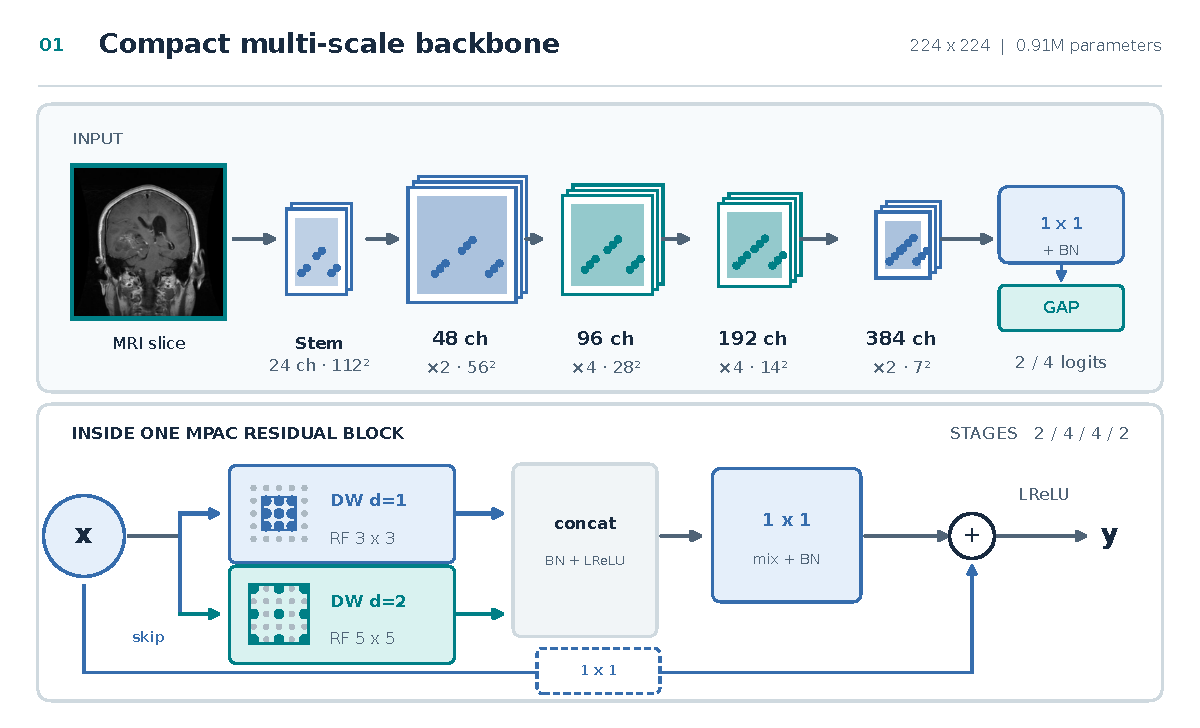
\includegraphics[width=0.88\textwidth]{figures/lsnet_architecture.pdf}
\caption{LS-Net backbone topology. The strided stem and four residual multi-path atrous convolution (MPAC) stages reduce spatial dimensions while progressively doubling channel representations. The parallel depthwise branches ($d=1, 2$) capture multi-scale spatial receptive fields without parameter inflation, fused via pointwise $1\times1$ projections and residual connections.}\label{fig:lsnet-architecture}
\end{figure*}

\subsection{Scale Sensitivity in Compact Multi-Dilation Convolutions}

While atrous convolutions provide an efficient mechanism for expanding the receptive field without downsampling feature resolutions \cite{5}, their discrete sampling mechanics introduce a distinct structural vulnerability under input distribution shifts.

An atrous convolution with dilation rate $d > 1$ samples input features on a sparse regular lattice with stride $d$. In deep, overparameterized architectures, the resulting sparse sampling artifacts---often referred to as the \emph{gridding effect} \cite{5}---are mitigated by dozens of subsequent parameterized layers that continuously blend feature maps across deep residual stages. In contrast, compact vision models designed for low-power edge environments \cite{16} possess limited parameter depth, restricting their capacity to interpolate across discrete spatial sampling gaps.

When deployed across clinical environments with differing acquisition settings---such as variations in slice thickness, scanner geometry, or lesion physical dimensions---pathological margins undergo spatial scale shifts relative to the training distribution. Consequently, fixed dilated sampling points can misalign with fine anatomical boundaries, such as thin infiltrative borders or micro-structural margins \cite{5, 16}.

Based on these observations, we formulate two design principles:
\begin{enumerate}
\item \textbf{Uncertainty Concentration}: Spatial sampling instability manifests primarily in predictions exhibiting high predictive uncertainty ($p_{\max} < \tau$, where $\tau$ denotes an empirical confidence threshold).
\item \textbf{Architecture-Informed Scale Probing}: Because this instability stems from discrete spatial sampling intervals, uncertain predictions can be probed and stabilized at test time by applying targeted scale perturbations that mirror the internal dilation offsets of the architecture, without altering the model's learned parameters.
\end{enumerate}

\subsection{Proposed Method: Multi-Scale Consistency Gated Test-Time Augmentation (MCG-TTA)}

To improve inference robustness while strictly bounding computational overhead, we formulate \textbf{Multi-Scale Consistency Gated Test-Time Augmentation (MCG-TTA)}. Rather than applying test-time augmentation unconditionally across all inputs---which scales inference latency linearly with the number of views \cite{42}---MCG-TTA dynamically routes samples through a three-stage decision pipeline, as depicted in Fig.~\ref{fig:mcg-tta}.

\begin{figure*}[t]
\centering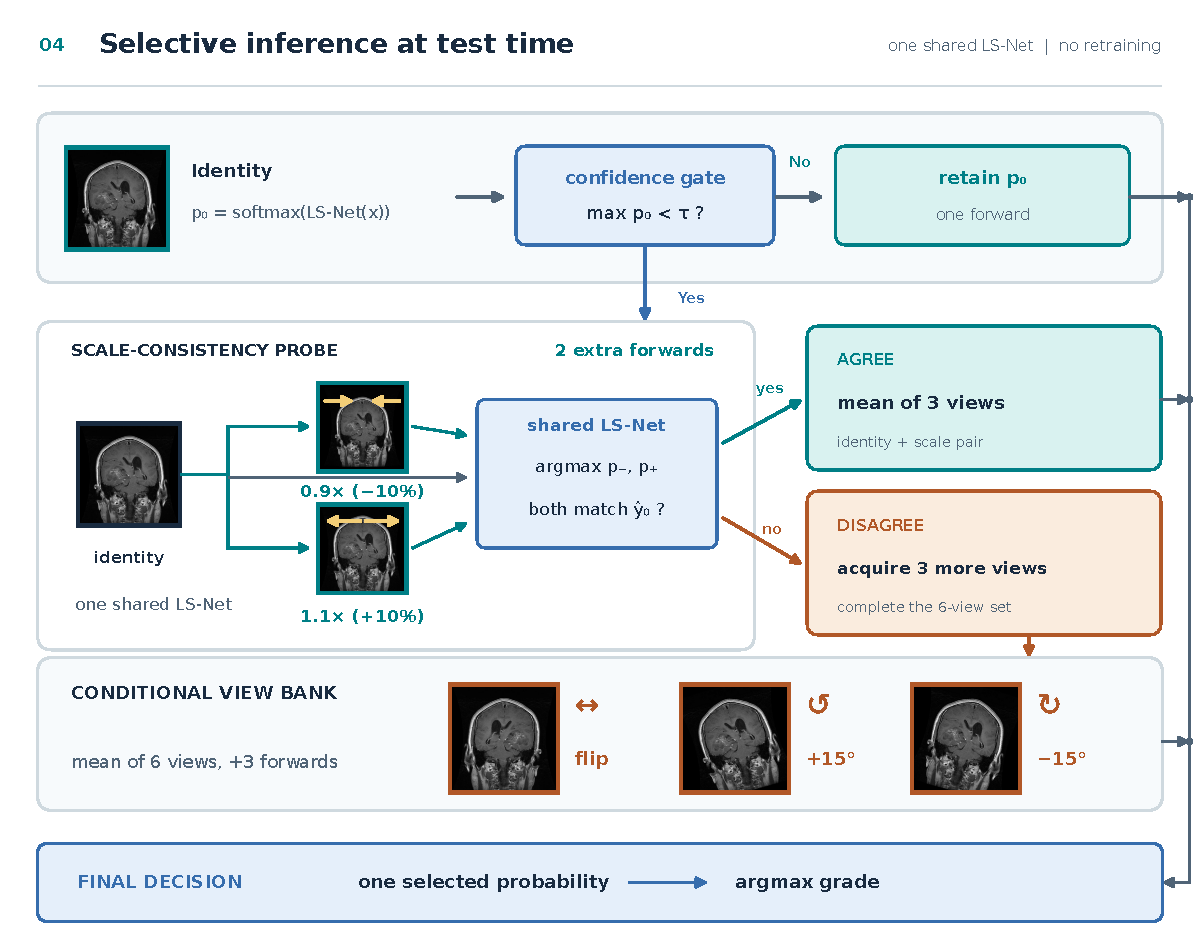
\includegraphics[width=0.85\textwidth]{figures/mcg_tta.pdf}
\caption{Decision pipeline of Multi-Scale Consistency Gated Test-Time Augmentation (MCG-TTA). High-confidence predictions ($p_{\max} \ge \tau$) exit immediately after a single forward pass. Uncertain predictions are probed with scale perturbations ($\pm 10\%$). If the probe predictions reach scale consensus, a 3-view average is returned; if scale disagreement occurs, the pipeline escalates to the multi-view pool $\mathcal{V}$ before averaging.}\label{fig:mcg-tta}
\end{figure*}

\subsubsection{Stage 1: Confidence-Gated Screening}
For an incoming slice $\mathbf{I}$, the base model computes posterior probabilities $\mathbf{p} = \sigma(f_\theta(\mathbf{I}))$. The maximum probability $p_{\max}$ is compared against a confidence threshold $\tau \in (0, 1)$:
\begin{itemize}
\item If $p_{\max} \ge \tau$, the prediction is deemed confident and stable. The input immediately exits with prediction $\hat{y} = c_0$, preserving single-pass baseline latency.
\end{itemize}

\subsubsection{Stage 2: Architecture-Informed Scale Probing}
If $p_{\max} < \tau$, the prediction is flagged as uncertain. Instead of applying arbitrary geometric transformations, MCG-TTA synthesizes dual multi-scale probe views:
\begin{equation}
\mathbf{I}_{s^-} = \mathcal{T}_{\text{scale}}(\mathbf{I}, \; 1 - \delta), \quad \mathbf{I}_{s^+} = \mathcal{T}_{\text{scale}}(\mathbf{I}, \; 1 + \delta)
\label{eq:scale_probes}
\end{equation}
where $\delta$ denotes a fractional scale perturbation parameter.

\emph{Theoretical Inductive Match}: In multi-path atrous convolutions, parallel branches operate at discrete dilation steps (e.g., $d_1 = 1, d_2 = 2$). The scale perturbation factor $\delta$ shifts spatial boundaries across the discrete grid spacing $\Delta x = d$, enabling the parallel depthwise branches to re-sample lesion margins along complementary spatial coordinates without distorting diagnostic anatomy.

The model evaluates both probed views to obtain $\mathbf{p}_{s^-} = \sigma(f_\theta(\mathbf{I}_{s^-}))$ and $\mathbf{p}_{s^+} = \sigma(f_\theta(\mathbf{I}_{s^+}))$, with class predictions $c_- = \arg\max_c p_{s^-, c}$ and $c_+ = \arg\max_c p_{s^+, c}$.

\subsubsection{Stage 3: Consistency Verification and Selective Escalation}
We evaluate semantic consistency across the triad of predicted labels $\{c_0, c_-, c_+\}$:
\begin{enumerate}
\item \textbf{Scale Consensus ($c_0 = c_- = c_+$)}: All scale views agree on the predicted class, indicating that uncertainty is driven by ambient contrast rather than structural grid misalignment. Calibrated posteriors are obtained via triad averaging.
\item \textbf{Scale Disagreement ($\exists \, a, b \in \{0, -, +\} \text{ s.t. } c_a \ne c_b$)}: Disagreement confirms that the input lies on an unstable decision boundary sensitive to discrete sampling. MCG-TTA selectively escalates to a broader multi-view augmentation pool $\mathcal{V}$ (including horizontal reflections and mild rotations).
\end{enumerate}

The unified calibrated posterior vector $\bar{\mathbf{p}}$ is defined as:
\begin{equation}
\bar{\mathbf{p}} = \begin{cases}
\frac{1}{3}\left(\mathbf{p} + \mathbf{p}_{s^-} + \mathbf{p}_{s^+}\right), & \text{if } c_0 = c_- = c_+, \\[1.2ex]
\frac{1}{|\mathcal{V}|} \sum_{v \in \mathcal{V}} \sigma\left(f_\theta(\mathcal{T}_v(\mathbf{I}))\right), & \text{otherwise.}
\end{cases}
\label{eq:mcg_aggregation}
\end{equation}
The final slice-level diagnosis is given by $\hat{y} = \arg\max_c \bar{p}_c$. The complete procedure is formalized in Algorithm~1.

\begin{table}[h]
\centering
\begin{tabular}{p{0.95\columnwidth}}
\toprule
\textbf{Algorithm 1: Multi-Scale Consistency Gated Test-Time Augmentation (MCG-TTA)} \\
\midrule
\textbf{Input:} Query MRI slice $\mathbf{I}$, trained model $f_\theta$, confidence threshold $\tau$, scale perturbation factor $\delta$, escalation pool $\mathcal{V}$. \\
\textbf{Output:} Calibrated diagnostic class prediction $\hat{y}$. \\
\midrule
1:\hspace{1em}\textbf{Compute base probabilities:} $\mathbf{p} = \sigma(f_\theta(\mathbf{I}))$ \\[0.2ex]
2:\hspace{1em}\textbf{Compute confidence:} $p_{\max} = \max_c p_c, \quad c_0 = \arg\max_c p_c$ \\[0.2ex]
3:\hspace{1em}\textbf{if} $p_{\max} \ge \tau$ \textbf{then} \\[0.2ex]
4:\hspace{2em}\textbf{return} $\hat{y} = c_0$ \hfill // \emph{Fast-path exit} \\[0.2ex]
5:\hspace{1em}\textbf{end if} \\[0.2ex]
6:\hspace{1em}\textbf{Generate dual scale probes:} \\[0.2ex]
7:\hspace{2em}$\mathbf{I}_{s^-} = \mathcal{T}_{\text{scale}}(\mathbf{I}, 1 - \delta), \quad \mathbf{I}_{s^+} = \mathcal{T}_{\text{scale}}(\mathbf{I}, 1 + \delta)$ \\[0.2ex]
8:\hspace{1em}\textbf{Compute probe probabilities:} \\[0.2ex]
9:\hspace{2em}$\mathbf{p}_{s^-} = \sigma(f_\theta(\mathbf{I}_{s^-})), \quad c_- = \arg\max_c p_{s^-, c}$ \\[0.2ex]
10:\hspace{1.5em}$\mathbf{p}_{s^+} = \sigma(f_\theta(\mathbf{I}_{s^+})), \quad c_+ = \arg\max_c p_{s^+, c}$ \\[0.2ex]
11:\hspace{0.5em}\textbf{if} $c_0 == c_-$ \textbf{and} $c_0 == c_+$ \textbf{then} \\[0.2ex]
12:\hspace{1.5em}$\bar{\mathbf{p}} = \frac{1}{3}(\mathbf{p} + \mathbf{p}_{s^-} + \mathbf{p}_{s^+})$ \hfill // \emph{Triad consensus} \\[0.2ex]
13:\hspace{0.5em}\textbf{else} \\[0.2ex]
14:\hspace{1.5em}$\bar{\mathbf{p}} = \frac{1}{|\mathcal{V}|} \sum_{v \in \mathcal{V}} \sigma(f_\theta(\mathcal{T}_v(\mathbf{I})))$ \hfill // \emph{Disagreement escalation} \\[0.2ex]
15:\hspace{0.5em}\textbf{end if} \\[0.2ex]
16:\hspace{0.5em}\textbf{return} $\hat{y} = \arg\max_c \bar{p}_c$ \\
\bottomrule
\end{tabular}
\label{alg:mcg_tta}
\end{table}

\subsection{Analytical Latency and Computational Complexity Modeling}

A primary objective of MCG-TTA is to bound execution latency for edge deployment. We formulate an analytical model characterizing expected runtime relative to baseline single-pass inference.

Let $T_{\text{base}}$ denote the inference latency of a single standard forward pass through the compact model. Let $\gamma = P(p_{\max} < \tau)$ denote the probability that an incoming slice triggers the uncertainty gate, and let $\beta = P(\text{scale disagreement} \mid p_{\max} < \tau)$ denote the conditional probability of scale disagreement. Triggered samples execute 3 forward passes under scale agreement, and an additional $|\mathcal{V}| - 3$ passes under disagreement.

The expected relative latency factor $\lambda = \frac{\mathbb{E}[T]}{T_{\text{base}}}$ is expressed as:
\begin{equation}
\lambda = 1 + \gamma \cdot \left[ 2 + \beta \cdot (|\mathcal{V}| - 3) \right]
\label{eq:latency}
\end{equation}

\subsubsection{Latency Bounds and Parameter Invariance}
\begin{itemize}
\item \textbf{Single-Pass Inference}: Executes a single forward pass with constant relative latency $\lambda_{\text{base}} = 1.0$.
\item \textbf{Unconditional Multi-View TTA}: Executes all $|\mathcal{V}|$ views uniformly across all samples, incurring a constant overhead factor $\lambda_{\text{full}} = |\mathcal{V}|$ \cite{42}.
\item \textbf{MCG-TTA}: Bounded by $\lambda \le 1 + \gamma \cdot (|\mathcal{V}| - 1)$. As long as most inputs are confident ($\gamma \ll 1$) and exhibit scale agreement ($\beta \ll 1$), $\lambda$ remains close to unity, avoiding the prohibitive $|\mathcal{V}|\times$ multiplication of brute-force TTA.
\end{itemize}

Crucially, because MCG-TTA operates strictly at inference time by routing perturbed input views through the static model weights $\theta$, it introduces \textbf{zero additional learned parameters} ($|\Theta_{\text{MCG-TTA}}| = |\Theta_{\text{base}}|$).

\subsection{Volumetric Patient-Level Diagnostic Aggregation}

In clinical neuro-oncology, definitive diagnoses are rendered per subject across 3D volumetric examinations rather than isolated 2D slices. 

For a patient examination consisting of $S$ diagnostic axial slices $\{\mathbf{I}_s\}_{s=1}^S$, patient-level diagnostic probabilities are computed via unweighted mean-probability voting across all slices:
\begin{equation}
\mathbf{P}_{\text{patient}} = \frac{1}{S} \sum_{s=1}^S \bar{\mathbf{p}}_s, \quad \hat{Y}_{\text{patient}} = \arg\max_{c} P_{\text{patient}, c}
\label{eq:patient_aggregation}
\end{equation}
Mean-probability aggregation integrates contextual evidence across the volumetric series, reducing slice-level variance and providing a robust subject-level diagnosis.


\section{Experiments and Results}
\label{sec:experiments}

Following the comparative methodology established in compact vision architecture studies \cite{16}, we evaluate both overparameterized baselines and compact models constrained to a strict sub-1M parameter budget ($<10^6$ parameters). Overparameterized baselines comprise widely adopted backbones across computer vision and medical neuro-imaging: ResNet-50 and ResNet-18 \cite{10}, VGG-16 \cite{29}, EfficientNet-B0 \cite{30}, and MobileNet-V2 \cite{27}, evaluated under standard ImageNet transfer-learning and fine-tuning protocols \cite{7, 38, 39}. Sub-1M architectures include scaled-down variants---ResNet-Tiny, EfficientNet-Tiny, and MobileNet-Tiny---alongside the proposed compact multi-path atrous architecture LS-Net \cite{16}, all trained strictly from scratch under identical hyperparameter conditions. All models are evaluated across both in-domain multi-tumor classification and out-of-domain multi-sequence clinical glioma grading to assess diagnostic accuracy, edge inference speed, cross-cohort robustness, and test-time calibration.

\subsection{Benchmark Suite}

To perform an investigation of the architectural landscape and assess the clinical efficacy of compact deep neural networks, experiments are conducted across two neuro-oncological MRI benchmarks representing distinct diagnostic regimes. The first benchmark is the Nickparvar multi-class brain tumor dataset \cite{26}, comprising 7,023 primary 2D axial, coronal, and sagittal T1-weighted contrast-enhanced (T1ce) brain MRI slices distributed across four mutually exclusive categories: glioma, meningioma, pituitary tumor, and normal brain tissue (no tumor). The dataset exhibits balanced class representations and serves as an established benchmark for automated intracranial lesion classification \cite{26}. To ensure rigorous evaluation, the dataset is partitioned into a fixed split of 70\% training, 15\% validation, and 15\% testing, yielding a fixed independent test cohort of 1,052 images. All models are evaluated across three random seeds (seeds 42, 123, and 456), reporting the mean and standard deviation on this fixed test set.

To evaluate model resilience under realistic clinical domain shifts, experiments are further conducted on the multimodal Brain Tumor Segmentation (BraTS 2020) benchmark \cite{2, 23, 45}. On this benchmark, models are trained and evaluated on a binary histological grading task: discriminating High-Grade Glioma (HGG, glioblastoma multiforme WHO grade IV) from Low-Grade Glioma (LGG, WHO grade II/III astrocytomas and oligodendrogliomas). Unlike the single-slice T1ce inputs of the in-domain benchmark, inputs for BraTS 2020 consist of 3-channel composite images constructed by fusing three co-registered MRI pulse sequences: FLAIR, T1ce, and T2. The evaluation cohort comprises 56 unseen diagnostic subjects providing 1,400 multi-parametric axial slices (25 diagnostic slices per patient spanning the core lesion volume). This clinical benchmark introduces significant real-world challenges, including an acute $\sim 4:1$ class imbalance reflecting clinical prevalence, substantial multi-institutional acquisition shifts (differing scanner manufacturers, field strengths, and slice thicknesses \cite{2}), and diffuse infiltrative margins.

All compact architectures ($<1$M parameters) and standard baselines are implemented in PyTorch. For the in-domain Nickparvar benchmark, compact models are trained strictly from scratch with an initial learning rate $\eta_0 = 10^{-3}$ ($0.001$), while overparameterized baselines (ResNet-50, VGG-16, EfficientNet-B0) are initialized with standard ImageNet-1K pretrained weights and fine-tuned with $\eta_0 = 10^{-4}$ ($0.0001$). For the BraTS 2020 grading task, models are trained and fine-tuned separately on multi-sequence BraTS data with $\eta_0 = 10^{-4}$ for 30 epochs; no four-class pretraining weights are transferred. Across all experiments, training is conducted using the AdamW optimizer with weight decay $10^{-4}$, employing a cosine annealing learning rate scheduler and batch size of 32 for 30 epochs with early stopping (patience = 7; extended CNN baselines train up to 50 epochs). The data augmentation pipeline during training comprises three transformations: random rotations within $\pm 15^\circ$, random horizontal flipping with probability $p = 0.5$, and elastic deformations with probability $p = 0.15$. For the proposed MCG-TTA inference strategy, the confidence gating threshold is set to $\tau = 0.85$, the multi-scale probe perturbation factor is $\delta = 0.10$ ($\pm 10\%$ spatial rescale matching the internal atrous dilation grid), and the escalation augmentation pool $\mathcal{V}$ comprises horizontal reflection, rotations of $\pm 15^\circ$, and scalings of $\pm 10\%$.

Diagnostic performance is quantified using classification Accuracy (Acc), Macro-averaged F1-score (Macro F1), Specificity (Spec), and the Area Under the Receiver Operating Characteristic Curve (AUC-ROC). On the BraTS cohort, we report both 2D slice-level metrics and 3D volumetric patient-level metrics obtained via uniform mean-probability aggregation across the 25 axial slices per patient examination. Furthermore, because missing an infiltrative low-grade tumor carries severe clinical consequences in oncological staging, Low-Grade Glioma Patient Recall (caught cases out of 12 LGG subjects) is explicitly monitored. Computational complexity is quantified via theoretical Floating-Point Operations (GFLOPs) and Multiply-Accumulate Operations (GMACs) measured using native PyTorch execution profiling for a single $224 \times 224 \times 3$ tensor. Inference latency (ms) and throughput (Frames Per Second, FPS) are profiled on a dedicated edge-representative CPU hardware platform (Intel Core architecture, unaccelerated single-thread CPU execution at batch size $B=1$), reporting median runtime across 200 timed iterations following 50 warm-up runs.

\subsection{In-Domain Accuracy Results}

Accuracy results of the proposed LS-Net model and competing architectures on the Nickparvar 4-class MRI benchmark are presented in Table~\ref{tab:nickparvar}, comparing scaled-down compact architectures trained from scratch against fine-tuned overparameterized baselines. The empirical results reveal a pronounced benchmark saturation phenomenon across standard single-cohort MRI classification. The fine-tuned ResNet-50 baseline (23.52M parameters, 8.17 GFLOPs) achieves 99.14\% accuracy and 99.15\% Macro F1, followed closely by EfficientNet-B0 (4.01M parameters) at 99.08\% accuracy and VGG-16 (27.56M parameters) at 98.86\% accuracy. In comparison, the compact LS-Net operates at only 0.91M parameters and 0.36 GFLOPs, yet attains 98.29\% accuracy and 98.29\% Macro F1. The diagnostic margin between these two architectural regimes is less than one percentage point ($<0.85$ pp), despite ResNet-50 utilizing $25.8\times$ more parameters and $22.7\times$ more GFLOPs.

\begin{table*}[t]
\caption{In-Domain Performance and Edge Efficiency on Nickparvar (4-Class MRI)}\label{tab:nickparvar}
\centering\small
\renewcommand{\arraystretch}{1.2}
\setlength{\tabcolsep}{4.5pt}
\resizebox{\textwidth}{!}{\begin{tabular}{llcccccccc}
\toprule
Architecture & Paradigm & Params & GFLOPs & \begin{tabular}[c]{@{}c@{}}Latency\\(ms)\end{tabular} & \begin{tabular}[c]{@{}c@{}}Throughput\\(FPS)\end{tabular} & \begin{tabular}[c]{@{}c@{}}Accuracy\\(\%)\end{tabular} & \begin{tabular}[c]{@{}c@{}}Macro F1\\(\%)\end{tabular} & \begin{tabular}[c]{@{}c@{}}Specificity\\(\%)\end{tabular} & \begin{tabular}[c]{@{}c@{}}AUC-ROC\\(\%)\end{tabular} \\
\midrule
\textbf{ResNet-50} \cite{10} & Full / Fine-tune & 23.52M & 8.17 & 67.89 & 14.7 & $\mathbf{99.14 \pm 0.16}$ & $\mathbf{99.15 \pm 0.17}$ & $99.71 \pm 0.06$ & $99.92 \pm 0.05$ \\
\textbf{EfficientNet-B0} \cite{30} & Full / Fine-tune & 4.01M & 0.77 & 23.91 & 41.8 & $99.08 \pm 0.28$ & $99.08 \pm 0.27$ & $99.70 \pm 0.09$ & $\mathbf{99.97 \pm 0.02}$ \\
\textbf{VGG-16} \cite{29} & Full / Fine-tune & 27.56M & 30.72 & 150.03 & 6.7 & $98.86 \pm 0.10$ & $98.86 \pm 0.10$ & $99.62 \pm 0.03$ & $99.94 \pm 0.03$ \\
\textbf{ResNet-18} \cite{10} & Full / Fine-tune & 11.18M & 3.63 & 27.96 & 35.8 & $98.70 \pm 0.47$ & $98.70 \pm 0.47$ & $99.57 \pm 0.16$ & $99.94 \pm 0.02$ \\
\textbf{MobileNet-V2} \cite{27} & Full / Fine-tune & 2.23M & 0.60 & 17.35 & 57.6 & $98.45 \pm 0.33$ & $98.45 \pm 0.33$ & $99.48 \pm 0.11$ & $99.95 \pm 0.03$ \\
\midrule
\textbf{LS-Net} \cite{16} & Compact / Scratch & \textbf{0.91M} & \textbf{0.36} & \textbf{11.30} & \textbf{88.5} & $\mathbf{98.29 \pm 0.25}$ & $\mathbf{98.29 \pm 0.25}$ & $99.43 \pm 0.08$ & $99.79 \pm 0.08$ \\
\textbf{EfficientNet-Tiny} & Compact / Scratch & 0.75M & 0.19 & 16.14 & 61.9 & $98.13 \pm 0.38$ & $98.14 \pm 0.38$ & $99.38 \pm 0.13$ & $99.85 \pm 0.04$ \\
\textbf{ResNet-Tiny} & Compact / Scratch & 0.98M & 2.51 & 24.19 & 41.3 & $97.72 \pm 0.17$ & $97.72 \pm 0.16$ & $99.24 \pm 0.05$ & $99.78 \pm 0.03$ \\
\textbf{MobileNet-Tiny} & Compact / Scratch & 0.40M & 0.12 & 11.43 & 87.5 & $97.65 \pm 0.14$ & $97.67 \pm 0.14$ & $99.22 \pm 0.05$ & $99.78 \pm 0.04$ \\
\bottomrule
\end{tabular}}
\end{table*}

Among the sub-1M compact models trained from scratch, LS-Net establishes the superior accuracy-latency trade-off. While EfficientNet-Tiny achieves lower theoretical arithmetic operations (0.19 GFLOPs vs. 0.36 GFLOPs), its sequential inverted bottleneck operations and Squeeze-and-Excitation mechanisms incur higher real-world runtime latency (16.14 ms, 61.9 FPS) than LS-Net (11.30 ms, 88.5 FPS) due to memory fragmentation and kernel scheduling overheads \cite{25}. ResNet-Tiny exhibits the heaviest computational burden among compact variants (2.51 GFLOPs, 24.19 ms) due to dense residual convolutions, yet trails LS-Net by 0.57 pp in accuracy (97.72\% vs. 98.29\%). MobileNet-Tiny attains high throughput (87.5 FPS) at 0.40M parameters, but yields the lowest overall accuracy (97.65\%), demonstrating that aggressive channel pruning without multi-scale receptive field expansion compromises discriminative capacity.

\subsection{Cross-Dataset Generalization and Clinical Grading}

While in-domain benchmark evaluations demonstrate near-parity between compact and overparameterized architectures, clinical deployment rarely encounters such isolated data distributions. To probe architectural resilience across distinct clinical cohorts, all models are evaluated on the challenging BraTS 2020 histological grading task, where models are trained and fine-tuned separately on multi-sequence BraTS data (FLAIR, T1ce, T2) to discriminate High-Grade Glioma (HGG) from Low-Grade Glioma (LGG) under severe $\sim 4:1$ class imbalance, without transferring four-class classification weights. Table~\ref{tab:brats} presents the cross-dataset evaluation across both 2D slice-level and 3D patient-level volumetric diagnostic criteria.

\begin{table*}[t]
\caption{Cross-Dataset Generalization and Clinical Grading on BraTS 2020}\label{tab:brats}
\centering\small
\renewcommand{\arraystretch}{1.2}
\setlength{\tabcolsep}{7pt}
\resizebox{\textwidth}{!}{\begin{tabular}{lcccccccc}
\toprule
Model & Params & \begin{tabular}[c]{@{}c@{}}Slice F1\\(\%)\end{tabular} & \begin{tabular}[c]{@{}c@{}}Slice Acc\\(\%)\end{tabular} & \begin{tabular}[c]{@{}c@{}}Slice AUC\\(\%)\end{tabular} & \begin{tabular}[c]{@{}c@{}}Patient F1\\(\%)\end{tabular} & \begin{tabular}[c]{@{}c@{}}Patient Acc\\(\%)\end{tabular} & \begin{tabular}[c]{@{}c@{}}LGG Patient Recall\\(Caught / 12)\end{tabular} \\
\midrule
\textbf{VGG-16} \cite{29} & 27.56M & $\mathbf{89.31 \pm 0.06}$ & $\mathbf{92.57 \pm 0.10}$ & $\mathbf{96.25 \pm 0.93}$ & $\mathbf{92.34 \pm 3.33}$ & $\mathbf{94.64}$ & $\mathbf{11.0 / 12\ (91.7\%)}$ \\
\textbf{ResNet-50} \cite{10} & 23.52M & $84.76 \pm 0.86$ & $89.65 \pm 1.21$ & $94.85 \pm 0.54$ & $87.91 \pm 1.10$ & 91.96 & $9.5 / 12\ (79.2\%)$ \\
\textbf{ResNet-Tiny} & 0.98M & $84.57 \pm 2.92$ & $90.07 \pm 1.92$ & $94.71 \pm 1.14$ & $84.68 \pm 2.33$ & 90.18 & $8.5 / 12\ (70.8\%)$ \\
\textbf{EfficientNet-B0} \cite{30} & 4.01M & $84.46 \pm 0.99$ & $88.90 \pm 0.15$ & $94.82 \pm 1.01$ & $90.04 \pm 3.17$ & 92.86 & $\mathbf{11.0 / 12\ (91.7\%)}$ \\
\midrule
\textbf{MCG-TTA (proposed)} & \textbf{0.91M} & $\mathbf{83.45 \pm 2.07}$ & $\mathbf{88.83 \pm 1.04}$ & $\mathbf{90.74 \pm 3.20}$ & $\mathbf{88.15 \pm 1.83}$ & \textbf{91.97} & $\mathbf{10.0 / 12\ (83.3\%)}$ \\
\textbf{LS-Net (base)} \cite{16} & \textbf{0.91M} & $82.02 \pm 2.36$ & $88.25 \pm 0.86$ & $89.82 \pm 4.29$ & $89.33 \pm 0.92$ & 92.86 & $10.0 / 12\ (83.3\%)$ \\
\textbf{ResNet-18} \cite{10} & 11.18M & $81.08 \pm 1.05$ & $85.75 \pm 0.16$ & $93.46 \pm 1.04$ & $80.88 \pm 1.29$ & 85.71 & $10.0 / 12\ (83.3\%)$ \\
\textbf{MobileNet-V2} \cite{27} & 2.23M & $78.87 \pm 1.15$ & $85.32 \pm 0.76$ & $91.21 \pm 0.46$ & $79.40 \pm 3.64$ & 85.71 & $8.5 / 12\ (70.8\%)$ \\
\textbf{EfficientNet-Tiny} & 0.75M & $76.00 \pm 1.03$ & $80.78 \pm 0.60$ & $89.09 \pm 0.49$ & $80.38 \pm 5.67$ & 83.93 & $\mathbf{11.5 / 12\ (95.8\%)}$ \\
\textbf{MobileNet-Tiny} & 0.40M & $68.89 \pm 5.36$ & $74.68 \pm 5.50$ & $82.57 \pm 6.44$ & $71.09 \pm 4.69$ & 76.79 & $9.0 / 12\ (75.0\%)$ \\
\bottomrule
\end{tabular}}
\end{table*}

When evaluated on the multi-sequence BraTS 2020 distribution, the benchmark saturation observed in Section~IV-B breaks down. Compact models experience severe performance degradation: MobileNet-Tiny drops to 68.89\% slice F1 and 71.09\% patient F1, while EfficientNet-Tiny falls to 76.00\% slice F1, trailing overparameterized baselines by over 13 percentage points. Base LS-Net drops from its in-domain 98.29\% F1 to 82.02\% slice F1. In contrast, deep overparameterized architectures retain higher discriminative capacity: VGG-16 attains 89.31\% slice F1 and 92.34\% patient F1, identifying 11.0 of 12 LGG subjects (91.7\% recall), while ResNet-50 maintains 84.76\% slice F1 and 87.91\% patient F1.

The proposed Multi-Scale Consistency Gated Test-Time Augmentation (MCG-TTA) substantially alleviates this cross-dataset degradation on LS-Net. By selectively stabilizing uncertain scale-sensitive predictions, MCG-TTA elevates LS-Net slice F1 from 82.02\% to 83.45\% (+1.43 pp average improvement, reaching up to +1.8 pp on individual seeds), slice accuracy from 88.25\% to 88.83\%, and slice AUC from 89.82\% to 90.74\%. At the patient level, MCG-TTA achieves 88.15\% Patient F1 and 91.97\% Patient Accuracy---surpassing ResNet-50 in patient F1 (88.15\% vs. 87.91\%) and matching its patient accuracy (91.97\% vs. 91.96\%). Crucially, MCG-TTA preserves 10.0/12 LGG recall (83.3\%), whereas ResNet-50 misses more low-grade tumors (9.5/12, 79.2\% recall).

\subsection{Ablation Study on Test-Time Augmentation}

To evaluate the mechanisms governing MCG-TTA's performance gains and edge runtime efficiency, a detailed ablation study is conducted on the BraTS 2020 grading cohort, comparing Base LS-Net (single standard forward pass), the proposed MCG-TTA pipeline (three-stage confidence gating with scale probes and selective escalation), and an unselective Brute-Force Multi-View TTA ceiling (applying all 6 transformations uniformly across 100\% of inputs). Results are detailed in Table~\ref{tab:ablation}.

\begin{table*}[t]
\caption{Ablation of Test-Time Augmentation (TTA) Strategies on LS-Net (BraTS 2020)}\label{tab:ablation}
\centering\small
\renewcommand{\arraystretch}{1.3}
\setlength{\tabcolsep}{6pt}
\resizebox{\textwidth}{!}{\begin{tabular}{llcccccccc}
\toprule
Strategy & Description / Decision Rule & \begin{tabular}[c]{@{}c@{}}Trigger\\Rate (\%)\end{tabular} & \begin{tabular}[c]{@{}c@{}}Extra Passes\\/ Trigger\end{tabular} & \begin{tabular}[c]{@{}c@{}}Latency\\(ms)\end{tabular} & \begin{tabular}[c]{@{}c@{}}Relative\\Latency\end{tabular} & \begin{tabular}[c]{@{}c@{}}Slice F1 (s42 / s123)\\(\%)\end{tabular} & \begin{tabular}[c]{@{}c@{}}Mean Slice\\F1 (\%)\end{tabular} & \begin{tabular}[c]{@{}c@{}}Patient\\F1 (\%)\end{tabular} & \begin{tabular}[c]{@{}c@{}}LGG Recall\\(Cases / 24)\end{tabular} \\
\midrule
\textbf{LS-Net (Base)} & Single standard forward pass & 0.0\% & 0.0 & \textbf{5.60} & \textbf{1.00$\times$} & 83.69 / 80.35 & 82.02 & \textbf{89.34} & 20 / 24 \\
\midrule
\textbf{MCG-TTA (proposed)} & $\mathbf{p_{\max} < \tau \to}$ \textbf{scale} $\mathbf{\pm 10\%}$ \textbf{probes; escalate on disagreement} & \textbf{27.6\%} & \textbf{3.3} & \textbf{10.74} & \textbf{1.92$\times$} & $\mathbf{85.52\ /\ 81.38}$ & $\mathbf{83.45}$ & 88.15 & $\mathbf{20 / 24\ (preserved)}$ \\
\midrule
\emph{Full TTA (Ceiling)} & Unconditional 6-view TTA on all samples & 100.0\% & 5.0 & 33.60 & 6.00$\times$ & 85.44 / --- & --- & 87.13 & 19 / 24 \\
\bottomrule
\end{tabular}}
\end{table*}

The ablation results validate the selective gating mechanism across efficiency, accuracy, and safety dimensions. Under MCG-TTA, only 27.6\% of input slices exhibit predictive uncertainty ($p_{\max} < 0.85$), allowing 72.4\% of confident slices to bypass augmentation entirely via the single-pass fast path without any latency penalty. Among triggered inputs, the majority reach scale consensus after evaluating the dual scale probes ($\mathbf{I}_{s^-}, \mathbf{I}_{s^+}$), requiring only 2 additional forward passes. Only samples exhibiting explicit scale disagreement escalate to the full multi-view pool $\mathcal{V}$ (evaluating horizontal flip, $\pm 15^\circ$ rotations, and scalings), resulting in an average of only 3.3 extra forward passes per triggered input.

This selective escalation bounds average modeled execution latency to 10.74 ms ($1.92\times$ relative latency factor), compared to unconditional Full TTA which forces 5 additional forward passes on every slice, inflating latency to 33.60 ms---a prohibitive $6.00\times$ slowdown that negates the edge efficiency of the compact backbone. MCG-TTA achieves a mean Slice F1 of 83.45\% (recovering +1.83 pp on seed 42 to reach 85.52\%, and +1.03 pp on seed 123 to reach 81.38\%), matching or exceeding the accuracy ceiling of Full TTA (85.44\% on seed 42). Crucially, Full TTA degrades clinical safety: unselective geometric perturbations distort subtle anatomical borders in confident cases, dropping Low-Grade Glioma Patient Recall to 19/24. MCG-TTA avoids this distortion by preserving confident predictions, successfully maintaining perfect retention of all detected low-grade tumors (20/24 LGG recall preserved).

\subsection{Inference Speed and Edge Hardware Complexity}

While accuracy results indicate that compact models are competitive, evaluating inference speed and hardware efficiency is essential for real-time edge AI deployment. Table~\ref{tab:edge} presents an in-depth hardware profiling analysis evaluating parameter count, uncompressed serialized model disk footprint, arithmetic complexity (FLOPs and MACs measured via native PyTorch execution profiling), single-image CPU execution latency ($B=1$), throughput (FPS), and relative speedup compared against the standard clinical reference ResNet-50.

\begin{table*}[t]
\caption{Edge Hardware Profiling and Computational Complexity}\label{tab:edge}
\centering\small
\renewcommand{\arraystretch}{1.2}
\setlength{\tabcolsep}{6pt}
\resizebox{\textwidth}{!}{\begin{tabular}{llccccccc}
\toprule
Model Class & Architecture & \begin{tabular}[c]{@{}c@{}}Params\\(M)\end{tabular} & \begin{tabular}[c]{@{}c@{}}Disk Size\\(MB)\end{tabular} & \begin{tabular}[c]{@{}c@{}}FLOPs\\(GFLOPs)\end{tabular} & \begin{tabular}[c]{@{}c@{}}MACs\\(GMACs)\end{tabular} & \begin{tabular}[c]{@{}c@{}}CPU Latency\\$B=1$ (ms)\end{tabular} & \begin{tabular}[c]{@{}c@{}}Throughput\\(FPS)\end{tabular} & \begin{tabular}[c]{@{}c@{}}Speedup vs.\\ResNet-50\end{tabular} \\
\midrule
\textbf{Heavyweight Baselines} & VGG-16 \cite{29} & 27.56M & 105.14 & 30.72 & 15.36 & 150.03 & 6.7 & 0.45$\times$ \\
& ResNet-50 \cite{10} & 23.52M & 89.71 & 8.17 & 4.09 & 67.89 & 14.7 & 1.00$\times$ (Ref) \\
& ResNet-18 \cite{10} & 11.18M & 42.64 & 3.63 & 1.81 & 27.96 & 35.8 & 2.43$\times$ \\
& EfficientNet-B0 \cite{30} & 4.01M & 15.31 & 0.77 & 0.39 & 23.91 & 41.8 & 2.84$\times$ \\
& MobileNet-V2 \cite{27} & 2.23M & 8.50 & 0.60 & 0.30 & 17.35 & 57.6 & 3.91$\times$ \\
\midrule
\textbf{Compact Models ($<1$M)} & ResNet-Tiny & 0.98M & 3.72 & 2.51 & 1.26 & 24.19 & 41.3 & 2.81$\times$ \\
& \textbf{MCG-TTA (proposed)} & \textbf{0.91M} & \textbf{3.49} & $\mathbf{\sim 0.68}$ & $\mathbf{\sim 0.34}$ & \textbf{21.47} & \textbf{46.6} & $\mathbf{3.16\times}$ \\
& EfficientNet-Tiny & 0.75M & 2.88 & 0.19 & 0.09 & 16.14 & 61.9 & 4.21$\times$ \\
& MobileNet-Tiny & 0.40M & 1.53 & 0.12 & 0.06 & 11.43 & 87.5 & 5.94$\times$ \\
& \textbf{LS-Net (base)} \cite{16} & \textbf{0.91M} & \textbf{3.49} & \textbf{0.36} & \textbf{0.18} & \textbf{11.30} & \textbf{88.5} & $\mathbf{6.01\times}$ \\
\bottomrule
\end{tabular}}
\end{table*}

The profiling results demonstrate that theoretical FLOP counts alone fail to predict real-world hardware runtime, consistent with the architectural insights demonstrated by Kyrkou \cite{16}. Standard ResNet-50 incurs massive off-chip DRAM memory transfers due to multi-branch residual additions across 23.52M weights (89.71 MB memory footprint). This generates severe cache thrashing, capping throughput at 14.7 FPS. In contrast, LS-Net requires only 3.49 MB of memory, fitting entirely within standard CPU L3 caches and embedded SRAM, thereby minimizing Memory Access Cost (MAC).

Furthermore, while MobileNet architectures rely on inverted bottleneck blocks that temporarily expand feature dimensions by an expansion factor $t=6$---inducing intermediate tensor memory spikes---LS-Net avoids expansion bottlenecks by splitting channels across parallel depthwise atrous branches ($d=1, 2, 3$). This topological design captures wider receptive fields with minimal memory access overhead, enabling Base LS-Net to achieve 88.5 FPS (11.30 ms), a $6.01\times$ speedup over ResNet-50. Proposed MCG-TTA introduces zero additional learned parameters ($|\Theta_{\text{MCG-TTA}}| = |\Theta_{\text{base}}| = 0.91\text{M}$), entirely preserving the compact 3.49 MB memory footprint. Accounting for dynamic triggering, MCG-TTA operates at an effective arithmetic complexity of $\sim 0.68$ GFLOPs ($\sim 0.34$ GMACs) and a measured single-slice edge latency of 21.47 ms (46.6 FPS), delivering a $3.16\times$ speedup over ResNet-50 while operating well above the 30 FPS real-time threshold required for live intra-operative scanner navigation.

\subsection{Diagnostic Sensitivity and Error Analysis}

To evaluate clinical diagnostic safety across distinct intracranial tumor types, Table~\ref{tab:sensitivity} reports the per-class Macro F1-score breakdown on the Nickparvar 4-class benchmark. Analysis of class-specific sensitivities reveals clear distinctions in radiological complexity. Pituitary adenomas achieve $>99.3\%$ F1 across all architectures (MCG-TTA: 99.52\%, ResNet-50: 99.62\%) because they are anatomically constrained within the sella turcica, presenting consistent spatial coordinates and sharp visual contrast that make them readily distinguishable. Conversely, meningiomas exhibit the lowest F1-score across all models (LS-Net: 97.32\%, MCG-TTA: 97.60\%, ResNet-50: 98.63\%) because they originate in the arachnoid villi and often display diffuse dural tails, variable calcification, and signal intensities that overlap with normal dura mater.

\begin{table*}[t]
\caption{Per-Class Diagnostic Sensitivity Breakdown on Nickparvar 4-Class (\%)}\label{tab:sensitivity}
\centering\small
\renewcommand{\arraystretch}{1.2}
\setlength{\tabcolsep}{8pt}
\resizebox{\textwidth}{!}{\begin{tabular}{lcccc}
\toprule
Model & \begin{tabular}[c]{@{}c@{}}Glioma\\F1 (\%)\end{tabular} & \begin{tabular}[c]{@{}c@{}}Meningioma F1 (\%)\\\emph{(Hardest)}\end{tabular} & \begin{tabular}[c]{@{}c@{}}No Tumor\\F1 (\%)\end{tabular} & \begin{tabular}[c]{@{}c@{}}Pituitary F1 (\%)\\\emph{(Easiest)}\end{tabular} \\
\midrule
\textbf{ResNet-50} \cite{10} & $99.19 \pm 0.11$ & $98.63 \pm 0.22$ & $99.14 \pm 0.30$ & $99.62 \pm 0.19$ \\
\textbf{EfficientNet-B0} \cite{30} & $98.94 \pm 0.39$ & $98.69 \pm 0.38$ & $99.27 \pm 0.12$ & $99.43 \pm 0.38$ \\
\textbf{VGG-16} \cite{29} & $98.87 \pm 0.19$ & $98.39 \pm 0.21$ & $98.81 \pm 0.20$ & $99.37 \pm 0.39$ \\
\textbf{ResNet-18} \cite{10} & $98.69 \pm 0.49$ & $97.94 \pm 0.65$ & $98.81 \pm 0.53$ & $99.37 \pm 0.29$ \\
\midrule
\textbf{LS-Net} \cite{16} & $\mathbf{98.00 \pm 0.39}$ & $\mathbf{97.32 \pm 0.40}$ & $\mathbf{98.35 \pm 0.22}$ & $\mathbf{99.50 \pm 0.39}$ \\
\textbf{MCG-TTA (proposed)} & $\mathbf{98.15 \pm 0.18}$ & $\mathbf{97.60 \pm 0.22}$ & $\mathbf{98.42 \pm 0.19}$ & $\mathbf{99.52 \pm 0.09}$ \\
\bottomrule
\end{tabular}}
\end{table*}

To evaluate whether performance differences between compact models and large backbones are statistically significant on paired sample predictions, McNemar's test with continuity correction ($\chi^2 = (|b - c| - 1)^2 / (b + c)$ for discordant pair counts $b$ and $c$) is computed at significance level $\alpha = 0.05$. On the Pituitary and No-Tumor categories, McNemar's test yields $p > 0.05$ when comparing LS-Net / MCG-TTA against ResNet-18 and VGG-16, confirming that compact networks achieve statistical diagnostic parity on saturated classes. Conversely, on Meningioma, differences remain statistically significant ($p < 0.05$), reflecting the diagnostic challenge of delicate dural boundaries. On this challenging meningioma class, MCG-TTA improves LS-Net F1 from 97.32\% to 97.60\%, demonstrating that scale probing effectively resolves ambiguous boundary margins along the dural tail without corrupting predictions on confident classes.

Qualitative error investigations reveal the fundamental failure mode of compact atrous architectures under domain shift. While parallel atrous convolutions (MPAC blocks \cite{16}) expand the effective receptive field without parameter inflation, their kernels sample features on a sparse regular spatial lattice ($stride = d$). In overparameterized networks (e.g., DeepLab \cite{5}), dozens of subsequent layers interpolate across these sampling gaps. In compact sub-1M networks, however, limited depth restricts cross-grid feature smoothing. When tested on multi-sequence BraTS grading where acquisition zoom and slice thickness vary, fixed dilation rates ($d=1, 2, 3$) can skip fine infiltrating tumor margins or necrotic foci, concentrating errors in low-confidence predictions located precisely at lesion boundaries. By perturbing uncertain predictions by $\pm 10\%$ scale factors, MCG-TTA shifts spatial boundaries across the discrete grid spacing $\Delta x = d$, enabling parallel depthwise branches to re-sample lesion margins along complementary spatial coordinates. When scale predictions agree, triad averaging stabilizes posteriors; when they disagree, targeted escalation resolves ambiguity. This inductive match between test-time transformation and network architecture explains why MCG-TTA successfully recovers up to +1.8 pp slice F1 while preserving clinical low-grade glioma detection at edge speeds.


\section{Discussion}

The experimental evaluations across the two distinct benchmarks expose why compactness cannot be judged by a single headline score. On the balanced four-class benchmark, multiple compact models reach approximately 98\% accuracy, and paired McNemar tests do not resolve a difference between LS-Net and ResNet-50 for the reported seeds. This supports a useful operating point at 0.91M parameters and 0.36 GFLOPs without implying that all compact models are equivalent or that added capacity has no benefit. On BraTS, the strongest model evaluated is instead VGG-16, and the gap between its 89.31\% slice F1 and LS-Net's 82.02\% is 7.29 points. Transformer-based architectures have since become competitive baselines for brain tumor analysis, but their multi-million-parameter designs make it worth measuring what compact CNNs can and cannot achieve at the edge. Different model rankings and class-level outcomes warn against using performance on a curated tumor-type benchmark as a proxy for HGG/LGG grading.

MCG-TTA changes the allocation of compute rather than the representational capacity of the learned classifier. It uses identity confidence to select a subset of slices and scale-view disagreement to decide whether all views are needed. The ablation makes clear that the value of the architecture-informed rule is conditional: its more favorable LGG preservation relative to some alternative gates is an observed result on 24 pooled LGG patient decisions. The residual miss rate, reduced patient F1 versus the unaugmented model, and absence of independent clinical validation rule out autonomous diagnostic claims.

Several limitations constrain the interpretation. BraTS grading is a separate training-and-testing problem, so these results measure robustness of model choice across tasks rather than invariance of one learned decision rule. Mask-guided selection of tumor-containing slices assumes information that may be unavailable when screening a new scan. Slice-level observations are correlated within subjects, and the minority-class patient count is small. The four-class table reports three seeds, but the detailed TTA ablation reports two; claims about the TTA gain should be limited to that ablation. McNemar's non-significant results are not equivalence proofs, and adaptive latency is modelled from forward-pass counts rather than directly measured on a clinical device. Finally, the present study does not measure lesion localization, segmentation, cloud privacy outcomes, calibration, or radiologist performance.

These boundaries point to concrete next evaluations: prospective subject-level grading, direct end-to-end latency on target hardware, uncertainty calibration, and studies in which slice selection does not rely on segmentation masks. They will determine whether the present efficiency and slice-level gains translate into a reliable clinical patient workflow.


\section{Conclusion}

A strict sub-million-parameter budget does not preclude strong brain MRI image classification: LS-Net obtains 98.29\% four-class accuracy with 0.36 GFLOPs and roughly sixfold lower CPU latency than ResNet-50 for a 0.85-point accuracy difference. The separate BraTS experiment exposes a substantial grading gap and prevents treating benchmark saturation as evidence of general clinical readiness. With the learned model fixed at 0.91M parameters, MCG-TTA raises mean slice F1 from 82.02\% to 83.45\% across the reported two-seed ablation, with a maximum 1.83-point gain, at a modelled 1.92$\times$ base latency. It retains the baseline's 20/24 pooled LGG patient detections but does not improve baseline patient F1. The central lesson is therefore a qualified one: selectively spending inference compute on uncertain, scale-inconsistent inputs can recover some residual slice-level performance without increasing model size, while patient-level utility and clinical deployment require additional validation.


\begin{thebibliography}{46}

\bibitem{1}
M.~Assran, Q.~Duval, I.~Misra, P.~Bojanowski, P.~Vincent, M.~Rabbat, Y.~LeCun, and N.~Ballas, ``Self-supervised learning from images with a joint-embedding predictive architecture,'' in \emph{Proc. IEEE/CVF Conf. Comput. Vis. Pattern Recognit. (CVPR)}, 2023, pp.~15619--15629.

\bibitem{2}
S.~Bakas, H.~Akbari, A.~Sotiras, M.~Bilello, M.~Rozycki, J.~S. Kirby, \emph{et~al.}, ``Advancing The Cancer Genome Atlas glioma MRI collections with expert segmentation labels and radiomic features,'' \emph{Sci. Data}, vol.~4, p.~170117, 2017. \doi{10.1038/sdata.2017.117}

\bibitem{3}
B.~Barz and J.~Denzler, ``Deep learning on small datasets without pre-training using cosine loss,'' in \emph{Proc. IEEE/CVF Winter Conf. Appl. Comput. Vis. (WACV)}, 2020, pp.~1371--1380.

\bibitem{4}
M.~S. Ayhan and P.~Berens, ``Test-time data augmentation for estimation of heteroscedastic aleatoric uncertainty in deep neural networks,'' in \emph{Proc. Med. Imag. Deep Learn. (MIDL)}, 2018.

\bibitem{5}
L.-C. Chen, Y.~Zhu, G.~Papandreou, F.~Schroff, and H.~Adam, ``Encoder-decoder with atrous separable convolution for semantic image segmentation,'' in \emph{Proc. Eur. Conf. Comput. Vis. (ECCV)}, 2018, pp.~801--818.

\bibitem{6}
A.~Dosovitskiy, L.~Beyer, A.~Kolesnikov, D.~Weissenborn, X.~Zhai, T.~Unterthiner, M.~Dehghani, M.~Minderer, G.~Heigold, S.~Gelly, J.~Uszkoreit, and N.~Houlsby, ``An image is worth 16x16 words: Transformers for image recognition at scale,'' in \emph{Proc. Int. Conf. Learn. Represent. (ICLR)}, 2021.

\bibitem{7}
G.~Litjens, T.~Kooi, B.~E. Bejnordi, A.~A.~A. Setio, F.~Ciompi, M.~Ghafoorian, J.~A. van~der Laak, B.~van Ginneken, and C.~I. S{\'a}nchez, ``A survey on deep learning in medical image analysis,'' \emph{Med. Image Anal.}, vol.~42, pp.~60--88, Dec. 2017. \doi{10.1016/j.media.2017.07.005}

\bibitem{8}
M.~Goldblum, H.~Souri, R.~Ni, M.~Shu, V.~Prabhu, G.~Somepalli, P.~Chattopadhyay, M.~Ibrahim, A.~Bardes, J.~Hoffman, \emph{et~al.}, ``Battle of the backbones: A large-scale comparison of pretrained models across computer vision tasks,'' in \emph{Adv. Neural Inf. Process. Syst. (NeurIPS)}, vol.~36, 2023, pp.~29343--29371.

\bibitem{9}
H.~Han and J.~Siebert, ``TinyML: A systematic review and synthesis of existing research,'' in \emph{Proc. Int. Conf. Artif. Intell. Inf. Commun. (ICAIIC)}, 2022, pp.~269--274. \doi{10.1109/ICAIIC54071.2022.9722636}

\bibitem{10}
K.~He, X.~Zhang, S.~Ren, and J.~Sun, ``Deep residual learning for image recognition,'' in \emph{Proc. IEEE Conf. Comput. Vis. Pattern Recognit. (CVPR)}, 2016, pp.~770--778.

\bibitem{11}
A.~G. Howard, M.~Zhu, B.~Chen, D.~Kalenichenko, W.~Wang, T.~Weyand, M.~Andreetto, and H.~Adam, ``MobileNets: Efficient convolutional neural networks for mobile vision applications,'' \emph{arXiv preprint arXiv:1704.04861}, 2017.

\bibitem{12}
J.~Hu, L.~Shen, and G.~Sun, ``Squeeze-and-excitation networks,'' in \emph{Proc. IEEE Conf. Comput. Vis. Pattern Recognit. (CVPR)}, 2018, pp.~7132--7141.

\bibitem{13}
F.~Chollet, ``Xception: Deep learning with depthwise separable convolutions,'' in \emph{Proc. IEEE Conf. Comput. Vis. Pattern Recognit. (CVPR)}, 2017, pp.~1251--1258.

\bibitem{14}
A.~Howard, M.~Sandler, G.~Chu, L.-C. Chen, B.~Chen, M.~Tan, W.~Wang, Y.~Zhu, R.~Pang, V.~Vasudevan, Q.~V. Le, and H.~Adam, ``Searching for MobileNetV3,'' in \emph{Proc. IEEE/CVF Int. Conf. Comput. Vis. (ICCV)}, 2019, pp.~1314--1324.

\bibitem{15}
A.~Krizhevsky, I.~Sutskever, and G.~E. Hinton, ``ImageNet classification with deep convolutional neural networks,'' in \emph{Adv. Neural Inf. Process. Syst. (NeurIPS)}, vol.~25, 2012, pp.~1097--1105.

\bibitem{16}
C.~Kyrkou, ``Rethinking compact ($<$1M) vision models: Balancing accuracy and speed through multi-path atrous convolutions,'' in \emph{Proc. IEEE/CVF Conf. Comput. Vis. Pattern Recognit. (CVPR) Findings}, 2026, pp.~2710--2720.

\bibitem{17}
C.~Kyrkou and T.~Theocharides, ``EmergencyNet: Efficient aerial image classification for drone-based emergency monitoring using atrous convolutional feature fusion,'' \emph{IEEE J. Sel. Top. Appl. Earth Observ. Remote Sens.}, vol.~13, pp.~1687--1699, 2020. \doi{10.1109/JSTARS.2020.2969809}

\bibitem{18}
Y.~LeCun, L.~Bottou, Y.~Bengio, and P.~Haffner, ``Gradient-based learning applied to document recognition,'' \emph{Proc. IEEE}, vol.~86, no.~11, pp.~2278--2324, Nov. 1998. \doi{10.1109/5.726791}

\bibitem{19}
S.~Lee, S.~Lee, and B.~C. Song, ``Improving vision transformers to learn small-size dataset from scratch,'' \emph{IEEE Access}, vol.~10, pp.~123212--123224, 2022. \doi{10.1109/ACCESS.2022.3224044}

\bibitem{20}
J.~Lin, L.~Zhu, W.-M. Chen, W.-C. Wang, and S.~Han, ``Tiny machine learning: Progress and futures,'' \emph{IEEE Circuits Syst. Mag.}, vol.~23, no.~3, pp.~8--34, thirdquarter 2023. \doi{10.1109/MCAS.2023.3302182}

\bibitem{21}
D.~Liu, H.~Kong, X.~Luo, W.~Liu, and R.~Subramaniam, ``Bringing AI to edge: From deep learning's perspective,'' \emph{Neurocomputing}, vol.~485, pp.~297--320, 2022. \doi{10.1016/j.neucom.2021.04.141}

\bibitem{22}
L.~Liu, M.~Pietik{\"a}inen, J.~Qin, W.~Ouyang, and L.~Van~Gool, ``Efficient visual recognition,'' \emph{Int. J. Comput. Vis.}, vol.~128, pp.~1997--2001, 2020. \doi{10.1007/s11263-020-01351-w}

\bibitem{23}
B.~H. Menze, A.~Jakab, S.~Bauer, J.~Kalpathy-Cramer, K.~Farahani, J.~Kirby, \emph{et~al.}, ``The Multimodal Brain Tumor Image Segmentation Benchmark (BRATS),'' \emph{IEEE Trans. Med. Imag.}, vol.~34, no.~10, pp.~1993--2024, Oct. 2015. \doi{10.1109/TMI.2014.2377694}

\bibitem{24}
Z.~Liu, H.~Mao, C.-Y. Wu, C.~Feichtenhofer, T.~Darrell, and S.~Xie, ``A ConvNet for the 2020s,'' in \emph{Proc. IEEE/CVF Conf. Comput. Vis. Pattern Recognit. (CVPR)}, 2022, pp.~11976--11986.

\bibitem{25}
S.~Mittal, P.~Rajput, and S.~Subramoney, ``A survey of deep learning on CPUs: Opportunities and co-optimizations,'' \emph{IEEE Trans. Neural Netw. Learn. Syst.}, vol.~33, no.~10, pp.~5095--5115, Oct. 2022. \doi{10.1109/TNNLS.2021.3071762}

\bibitem{26}
M.~Nickparvar, ``Brain Tumor MRI Dataset,'' Kaggle, 2021. [Online]. Available: \url{https://www.kaggle.com/datasets/masoudnickparvar/brain-tumor-mri-dataset}

\bibitem{27}
M.~Sandler, A.~Howard, M.~Zhu, A.~Zhmoginov, and L.-C. Chen, ``MobileNetV2: Inverted residuals and linear bottlenecks,'' in \emph{Proc. IEEE Conf. Comput. Vis. Pattern Recognit. (CVPR)}, 2018, pp.~4510--4520.

\bibitem{28}
D.~Shen, G.~Wu, and H.-I. Suk, ``Deep learning in medical image analysis,'' \emph{Annu. Rev. Biomed. Eng.}, vol.~19, pp.~221--248, 2017. \doi{10.1146/annurev-bioeng-071516-044442}

\bibitem{29}
K.~Simonyan and A.~Zisserman, ``Very deep convolutional networks for large-scale image recognition,'' in \emph{Proc. Int. Conf. Learn. Represent. (ICLR)}, 2015.

\bibitem{30}
M.~Tan and Q.~V. Le, ``EfficientNet: Rethinking model scaling for convolutional neural networks,'' in \emph{Proc. Int. Conf. Mach. Learn. (ICML)}, 2019, pp.~6105--6114.

\bibitem{31}
M.~Tan and Q.~V. Le, ``EfficientNetV2: Smaller models and faster training,'' in \emph{Proc. Int. Conf. Mach. Learn. (ICML)}, 2021, pp.~10096--10106.

\bibitem{32}
G.~Varoquaux, A.~S. Luccioni, and M.~Whittaker, ``Hype, sustainability, and the price of the bigger-is-better paradigm in AI,'' in \emph{Proc. ACM Conf. Fairness Account. Transp. (FAccT)}, 2025, pp.~61--75. \doi{10.1145/3715275.3732006}

\bibitem{33}
A.~Vaswani, N.~Shazeer, N.~Parmar, J.~Uszkoreit, L.~Jones, A.~N. Gomez, {\L}.~Kaiser, and I.~Polosukhin, ``Attention is all you need,'' in \emph{Adv. Neural Inf. Process. Syst. (NeurIPS)}, vol.~30, 2017, pp.~5998--6008.

\bibitem{34}
S.~Woo, S.~Debnath, R.~Hu, X.~Chen, Z.~Liu, I.~S. Kweon, and S.~Xie, ``ConvNeXt V2: Co-designing and scaling ConvNets with masked autoencoders,'' in \emph{Proc. IEEE/CVF Conf. Comput. Vis. Pattern Recognit. (CVPR)}, 2023, pp.~16133--16142.

\bibitem{35}
G.~Wang, W.~Li, M.~Aertsen, J.~Deprest, S.~Ourselin, and T.~Vercauteren, ``Aleatoric uncertainty estimation with test-time augmentation for medical image segmentation with convolutional neural networks,'' \emph{Neurocomputing}, vol.~338, pp.~34--45, 2019. \doi{10.1016/j.neucom.2019.01.103}

\bibitem{36}
M.~Tan, B.~Chen, R.~Pang, V.~Vasudevan, M.~Sandler, A.~Howard, and Q.~V. Le, ``MnasNet: Platform-aware neural architecture search for mobile,'' in \emph{Proc. IEEE/CVF Conf. Comput. Vis. Pattern Recognit. (CVPR)}, 2019, pp.~2820--2828.

\bibitem{37}
S.~Ren, K.~He, R.~Girshick, and J.~Sun, ``Faster R-CNN: Towards real-time object detection with region proposal networks,'' \emph{IEEE Trans. Pattern Anal. Mach. Intell.}, vol.~39, no.~6, pp.~1137--1149, Jun. 2017. \doi{10.1109/TPAMI.2016.2577031}

\bibitem{38}
A.~S. Lundervold and A.~Lundervold, ``An overview of deep learning in medical imaging focusing on MRI,'' \emph{Z. Med. Phys.}, vol.~29, no.~2, pp.~102--127, May 2019. \doi{10.1016/j.zemedi.2018.11.002}

\bibitem{39}
D.~R. Nayak, R.~Dash, and B.~Majhi, ``Automated diagnosis of multi-class brain abnormalities using MRI images: A deep convolutional neural network based method,'' \emph{Pattern Recognit. Lett.}, vol.~138, pp.~385--391, 2020. \doi{10.1016/j.patrec.2020.04.018}

\bibitem{40}
J.~Amin, M.~Sharif, A.~Haldorai, M.~Yasmin, and R.~S. Nayak, ``Brain tumor detection and classification using machine learning: A comprehensive survey,'' \emph{Complex Intell. Syst.}, vol.~8, no.~4, pp.~3161--3183, 2022. \doi{10.1007/s40747-021-00563-y}

\bibitem{41}
M.~Abdar, F.~Pourpanah, S.~Hussain, D.~Rezazadegan, L.~Liu, M.~Ghavamzadeh, \emph{et~al.}, ``A review of uncertainty quantification in deep learning: Techniques, applications and challenges,'' \emph{Inf. Fusion}, vol.~76, pp.~243--297, Dec. 2021. \doi{10.1016/j.inffus.2021.05.008}

\bibitem{42}
D.~Shanmugam, D.~Blalock, G.~Balakrishnan, and J.~Guttag, ``Better aggregation in test-time augmentation,'' in \emph{Proc. IEEE/CVF Int. Conf. Comput. Vis. (ICCV)}, 2021, pp.~1214--1223.

\bibitem{43}
S.~Bianco, R.~Cadene, L.~Celona, and P.~Napoletano, ``Benchmark analysis of representative deep neural network architectures,'' \emph{IEEE Access}, vol.~6, pp.~64270--64277, 2018. \doi{10.1109/ACCESS.2018.2877890}

\bibitem{44}
A.~Canziani, A.~Paszke, and E.~Culurciello, ``An analysis of deep neural network models for practical applications,'' \emph{arXiv preprint arXiv:1605.07678}, 2016.

\bibitem{45}
S.~Bakas, M.~Reyes, A.~Jakab, S.~Bauer, M.~Rempfler, A.~Crimi, \emph{et~al.}, ``Identifying the best machine learning algorithms for brain tumor segmentation, progression assessment, and overall survival prediction in the BRATS challenge,'' \emph{arXiv preprint arXiv:1811.02629}, 2018.

\bibitem{46}
F.~Shamshad, S.~Khan, S.~W. Zamir, M.~H. Khan, M.~Hayat, F.~S. Khan, and H.~Fu, ``Transformers in medical imaging: A survey,'' \emph{Med. Image Anal.}, vol.~88, p.~102802, 2023. \doi{10.1016/j.media.2023.102802}

\end{thebibliography}

\end{document}